% !TEX root = ./repair.tex
\let\epsilon\varepsilon
\def\point#1{\vskip10pt\noindent{\it\bfseries #1.}\enspace}
\def\L{{\mathcal L}}

\section{Problem formulation and overview of results}
\label{sec:overview}

In this section we formulate the problem of model repair, and give an overview of our results. Suppose that $\hat\theta \in \reals^p$ is a model with $p$ parameters estimated on $n$ data points $\{(x_i, y_i)\}_{i=1}^n$ as a classification or regression model. The model $\hat\theta$ is then corrupted by noise. The primary noise model we study in this paper is
\begin{equation}
  \eta = \hat\theta + z
\end{equation}
where $z_j \sim (1-\epsilon) \delta_0 + \epsilon Q_j$ and $Q_j$ is an arbitrary distribution. In other words, each component $\hat\theta_j$ of $\hat\theta$ is corrupted by additive noise from an arbitrary distribution $Q_j$ with probability $\epsilon$, where $0\leq \epsilon \leq 1$, and is uncorrupted with probability $1-\epsilon$. We discuss alternative error models later in the paper. The goal is to recover $\hat\theta$ from $\eta$, without reestimating the model using the response values $\{y_i\}$.

\point{Overparameterized linear models}
To explain the main ideas, let us first consider the setting of under-determined linear regression. Let $X\in\reals^{n\times p}$ be the design matrix and $y\in\reals^n$ a vector of response values, and suppose that we wish to minimize the squared error  $\|y-X\theta\|_2^2$. If $n > p$ then this is an under-determined optimization problem. Among all solutions to the linear system $y = X\theta$, the solution of minimal norm $\|\theta\|_2$ is given by
\begin{equation}
  \hat \theta = X^T (X X^T)^{-1} y \label{eq:min-norm-solution}
\end{equation}
assuming that $X$ has full rank $n$ \citep{boyd:04}. Thus, $\hat\theta$ lies in the row space of the $n\times p$ design matrix $X$.

Now suppose that $\eta = \hat\theta + z$ where $z_j \sim (1-\epsilon) \delta_0 + \epsilon Q_j$. The method we propose to recover $\hat\theta$ from $\eta$ is to let $\tilde u\in\reals^n$ be the solution to the optimization
\begin{equation}
  \tilde u = \argmin_u \| \eta  - X^T u\|_1
  \label{eq:keylp}
\end{equation}
and define the repaired model as $\tilde\theta = X^T\tilde u$.
The linear program defined in \eqref{eq:keylp} can be thought of as performing median regression of $\eta$ onto the rows of $X$.
Our analysis shows that, under appropriate assumptions, the model is repaired with high probability, so that $\tilde \theta = \hat\theta$, as long as $n/p \leq c(1-\epsilon)^2$ for some sufficiently small constant $c$.

Figure~\ref{fig:exp} shows the performance of
the repair algorithm in simulation. The design is sampled as $X_{ij} \sim N(0,1)$ and the corruption distribution is $Q_j = N(1,1)$ for each $j$. With the sample size fixed at $n=50$, the dimension $p$ is varied according to $p_k/n=200/k^2$ with
$k$ ranging from 1 to 6. The plots show the empirical probability of exact repair $\tilde\theta = \hat\theta$ as a function of $\epsilon$. The roughly equal spacing of the curves agrees with our theory, which indicates that $\sqrt{n/p}/(1-\epsilon)$ should be sufficiently small for successful repair. The theory indicates that the repair probability for dimension $p_k$ as a function of the adjusted value $\epsilon_k = \epsilon + c'\cdot k - \frac{1}{2}$ should exhibit a threshold at
$\epsilon_k = 1/2$ for the constant $c' = \frac{\sqrt{2}}{20 c}$; this is seen in the right plot of Figure~\ref{fig:exp}.



\point{Robust regression} This procedure can be viewed in terms of robust regression. Specifically, $\eta$ can be viewed as a corrupted response vector, and $A = X^T \in \reals^{p\times n}$ can be viewed as design matrix that is \textit{not corrupted}.  Our result makes precise conditions under which this robust regression problem can be successfully carried out.
In particular, we show that model repair is possible even if $\epsilon \to 1$, so that the proportion of corrupted model components approaches one. This is in stark contrast to the traditional Huber model where the design is corrupted \citep{huber:64}, under which consistent estimation is only possible if $\epsilon \to 0$ \citep{chen2016,gao2020}.

\begin{figure}[t]
  \begin{tabular}{cc}
    \hskip-3pt
    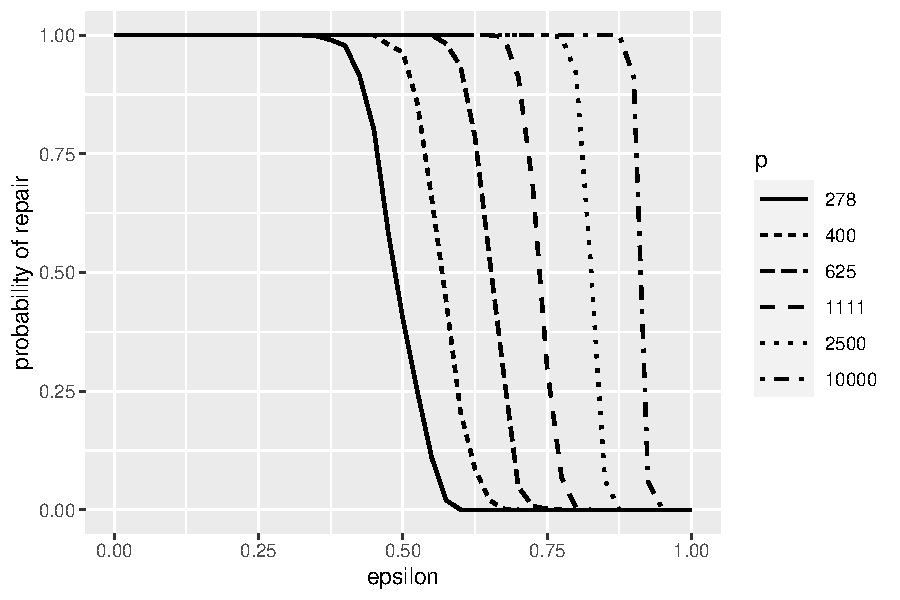
\includegraphics[width=.48\textwidth]{fig/plot-linear-50} &
    \hskip-3pt
    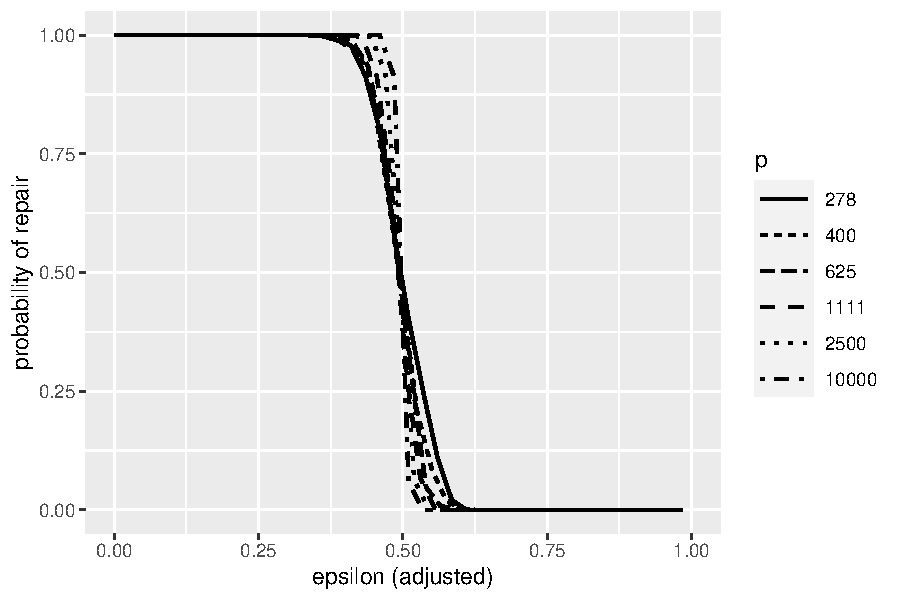
\includegraphics[width=.48\textwidth]{fig/plot-linear-50-adj}
  \end{tabular}
\caption{Left: Empirical probability of exact repair as a function of $\epsilon$.
The sample size is $n=50$ and the model dimension $p$
varies as $p_k/n = 200 /k^2$, for $k=1,\ldots, 6$; each point is an average over 500 trials. The plot on the right
shows the repair probability as a function of the adjusted value $\epsilon_k = \epsilon + c' \cdot k - \frac{1}{2}$
for dimension $p_k$, where the constant is $c'=\frac{\sqrt{2}}{20 c}=0.085$.}
\label{fig:exp}
\end{figure}

\point{Error-correcting codes}
Model repair can also be viewed in terms of error-correcting codes. Specifically, viewing the response vector $y\in\reals^n$  as a ``message'' to be communicated over a noisy channel, the minimum norm model $\hat\theta = X^T u = X^T (X X^T)^{-1} y$ redundantly
encodes $y$ since $p > n$ (see Figure~\ref{fig:code}). The decoding algorithm $\tilde u = \argmin_u \|\eta - X^T u\|$ then recovers the data $y$ according to $y = (XX^T) \tilde u$. The inequality $n/p < c(1-\epsilon)^2$ gives a condition on the rate of the code, that is, the level of redundancy that is sufficient for this decoding procedure to recover the message with high probability.

When $X$ is a random Gaussian matrix, the mapping $u \to X^T u = \sum_{i=1}^n u_i X_i^T$ can be viewed as a superposition of random codewords in $\reals^p$ \citep{joseph2012,rush2017}. The fundamental difference with channel coding is that in our regression setting the design matrix $X$ is fixed, and is not chosen for optimal channel coding. Indeed, the noise model $w \to w + z$ that we consider corresponds to a channel having infinite capacity, and a simple repetition code would suffice for identifying components that are uncorrupted \citep{CoverThomas}.

\begin{figure}[t]
  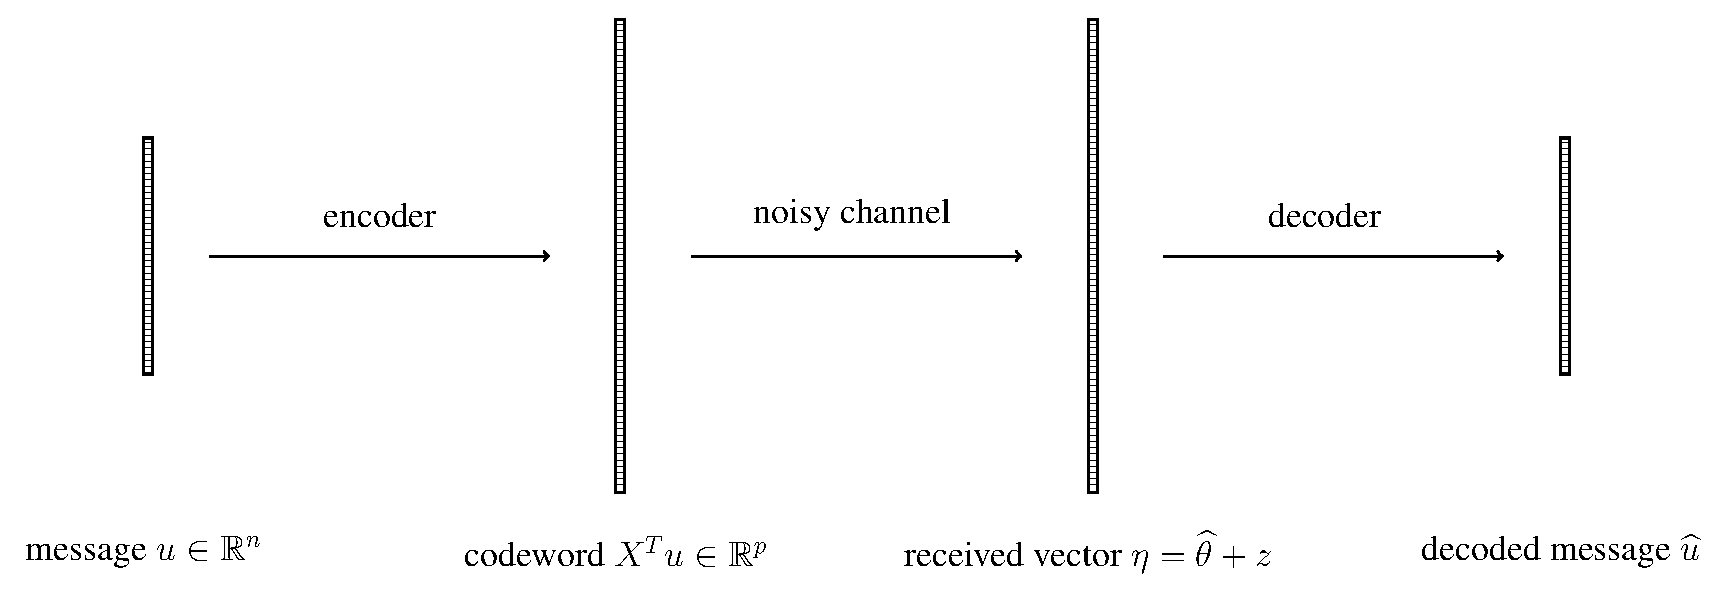
\includegraphics[width=1.0\textwidth]{fig/code}
  \caption{Model repair viewed in terms of error-correcting codes. The model $\hat\theta = X^T u\in\reals^p$ is in the row-space of the design matrix, which gives a redundant representation of the ``message'' $u\in\reals^n$ for $n < p$. The model is received as a noisy version $\eta$ with each entry corrupted with probability $\epsilon$. The received vector is decoded by solving a linear program.}
  \label{fig:code}
\end{figure}

\point{Estimators based on gradient descent}
The observations made above carry over to estimators of linear models based on gradient descent and stochastic gradient descent for arbitrary loss functions. Consider objective functions of the form
\begin{equation}
  \ell(\theta) = \frac{1}{n} \sum_{i=1}^n \L(y_i, x_i^T \theta)\label{eq:gen-obj}
\end{equation}
where $\L(y,f)$ is a general loss function; this includes
a broad range of estimators for problems such as linear least squares and logistic regression, robust regression, support vector machines, and others. The gradient descent update rule is
\begin{align}
  \theta^{(t+1)} &= \theta^{(t)} - \gamma_t \frac{1}{n} \sum_{i=1}^n \nabla_\theta \L(y_i, x_i^T \theta^{(t-1)}) \\
  &= \theta^{(t)} - \gamma_t \frac{1}{n} \sum_{i=1}^n \frac{\partial}{\partial f} \L(y_i, x_i^T \theta^{(t-1)}) x_i \\
  &= \theta^{(t)} - \sum_{i=1}^n w_i^{(t)} x_i
\end{align}
where $\gamma_t$ is a step size parameter. If the model is initialized at $\theta^{(0)}= 0\in\reals^p$ then the estimate at time $t$ can thus be written as
\begin{equation}
  \theta^{(t)} = X^T u^{(t)}
\end{equation}
for some $u^{(t)}\in \reals^n$. After contamination, we have $\eta = X^T u^{(t)} + z$. Therefore, we can recover the model
by computing  $\tilde\theta = X^T \tilde u$ where $\tilde u$ is the solution to \eqref{eq:keylp}.


The same conclusion holds for estimators based on stochastic gradient descent. With $B_t$ denoting the set of samples used in the mini-batch of the $t$th iteration, we can write
\begin{equation}
  \theta^{(t)} = \sum_{i\in B_1\cup\cdots\cup B_t} u_i^{(t)} x_i.
\end{equation}
We can recover $\theta^{(t)}$ from a corrupted model $\eta$ by computing $\tilde \theta = X^T_{B_1\cup \cdots B_t} \tilde u$ with
\begin{equation}
  \tilde u = \argmin_u \| \eta - X^T_{B_1\cup \cdots B_t} u\|_1
\end{equation}
where the submatrix $X_{B_1\cup\cdots B_t}$ only includes rows of $X$ for indices that were visited during some stochastic
gradient descent step. Our theory then establishes that the model is recovered with high probability in case
\begin{equation}
  \frac{\sqrt{{|B_1 \cup \cdots B_t|}/{p}}}{1-\epsilon} < c.
\end{equation}
Typically the training takes place in ``epochs'' where all $n$ data points are visited in each epoch.

\point{Random features and neural networks} Our theory extends to random features models \citep{rahimi2008}, where the covariates are $\tilde X = \psi(X W)\in \reals^{n\times p}$ where $X\in\reals^{n\times d}$, the matrix $W\in\reals^{d\times p}$ is a random Gaussian matrix that is not trained, and $\psi$ is a threshold function such as the hyperbolic tangent function or rectified linear unit. In particular, when the model is trained using gradient descent, the parameters $\hat\theta$ lie in the row
space of the matrix $\tilde X$. We also show how the ideas can be extended to neural networks, where the weights $W$ are trained. This requires modifications to the training and recovery algorithms that we detail below.
